\section{Methods and Materials}
\label{methods}
\subsection{Experimental Design}
\subsection{Ethical Clearance}
\label{methods_ethical}
As with any project involving humans, the details of the project must be reviewed and 
approved by the University Human Ethics Committee prior to any student participation.

An application for review was submitted in June and approved with modifications
on 25 July 2012 in time for the second week of semester.

The application included details of the methods of data collection, recruitment of participants,
and approval by a `Gatekeeper' who provides access to participants - in this case the course coordinator of JAPN1023, Dr Yuriko Nagata.

Data was to be stored anonymously and securely. In order to ensure participation was anonymous,
cards containing unique codes were to be handed out randomly to participants to allow them to
register online. Student review data was tied to a unique number in the database which could
not be traced back to individual students. Email addresses were collected from students in order
to allow them to log in and to reset their password if required, however exported review data was
stored only against a unique number in the database which could not be traced back to individual
students. Participants were also given an information sheet (See Appendix
\ref{appendix_participant_info_sheet}) and a consent form (See Appendix
\ref{appendix_participant_consent_form}) to sign and return before receiving a registration card.

\subsection{Software Design}
\label{methods_softwaredesign}
\subsubsection{Requirements}

\subsubsection{Tools}
This section outlines the software tools that will be used for the project and reasoning for
choosing these tools.
\paragraph{Git and Github}
(\url{http://git-scm.com/}),
(\url{http://www.github.com/})

Git is a distributed version control system (VCS) which tracks changes
to source code (often amongst multiple developers) and keeps a complete history
of changes. This is invaluable when a change in code occurs that results in a critical
bug. Versions can be compared to find the change that introduced the bug, and production
code can be reverted if need be \cite{scott_chacon_pro_2009}.

Git repositories can be hosted anywhere, however Github offers free Git repository hosting
for open source projects. It also allows
users to 'fork' public repositories to create their own version of a project. For this
reason it is useful for research projects as the project can be picked up and continued
at any time by others.

Git was selected for this project because of its portability (moving repositories
between servers is trivial). Github was chosen as it is free, encourages collaboration and is also the tool of choice for the 
Centre of Educational Innovation in Technology \cite{zornig_ceit_2012} under which this project was completed. 

\paragraph{Ruby on Rails}
(\url{http://www.rubyonrails.org/})

Ruby on Rails (aka Rails) is a popular open source framework for developing web applications\cite{bachle_ruby_2007}.
Rails was originally extracted from a commercial application (Basecamp by 37Signals) to create a generic
application framework \cite{carneiro_jr._beginning_2010} written in the Ruby language. Rails is designed for
rapid development and provides many guidelines which the developer is recommended to follow in order to speed up
development. Additionally, as an open source project Rails has gained many developers who have contributed back
to the community by sharing reusable components (known as Ruby Gems) with the community. This means many pieces of
functionality can be used in a project without rewriting, speeding up the development process. Gems used in this
project include:
\begin{description}
\item[Prawn] Provides PDF output - used for generating registration code cards
\item[CanCan] User authorisation - Allow and deny access to users based on their role (participant, administrator, teacher)
\item[Highcharts-Rails] Adds the Highcharts library to the application (See section below)
\end{description}

% TODO Complete Rails section

\paragraph{Heroku}
(\url{http://www.heroku.com/})

Heroku is a private company offering hosting for Ruby on Rails applications with automated deployment. While deploying
a Rails application on a server normally requires system administrator knowledge and a significant amount of
time to install, Heroku
allows deployment via Git and automatically installs dependencies to get an application up and running in less
than a minute.

Heroku was chosen over a private server for this project since it was necessary to be able to push updates
to the live application quickly in order to respond to bugs and to reduce time spent finding faults in the server.

% TODO Complete Heroku section

\paragraph{Backbone.JS}
(\url{http://www.backbonejs.org/})
Backbone.js is an open source Javascript framework providing a model oriented structure for web applications.
It was selected because\ldots

% TODO Complete Backbone section

\paragraph{Highcharts}
(\url{http://www.highcharts.com/})

Highcharts is a commercial Javascript framework which provides graphing capabilities to web sites. Highcharts
allows free usage by non-commercial projects. Highcharts was selected for graphing usage statistics
on the website because of the features it provides in addition to recommendations on websites such as Stack Overflow \cite{stackoverflow_highcharts_2012}.
% TODO Complete Highcharts section

\paragraph{Twitter Bootstrap}
(\url{http://twitter.github.com/bootstrap})

Twitter Bootstrap is a set of default styles for websites and web applications, provided as open-source by Twitter. Using Twitter Bootstrap rapidly speeds up theming of a web application with default looks for navigation, buttons, text and layout.


See figure \ref{twitterbootstrap} for a comparison of default styling with and without Twitter Bootstrap
\begin{figure}[h!]
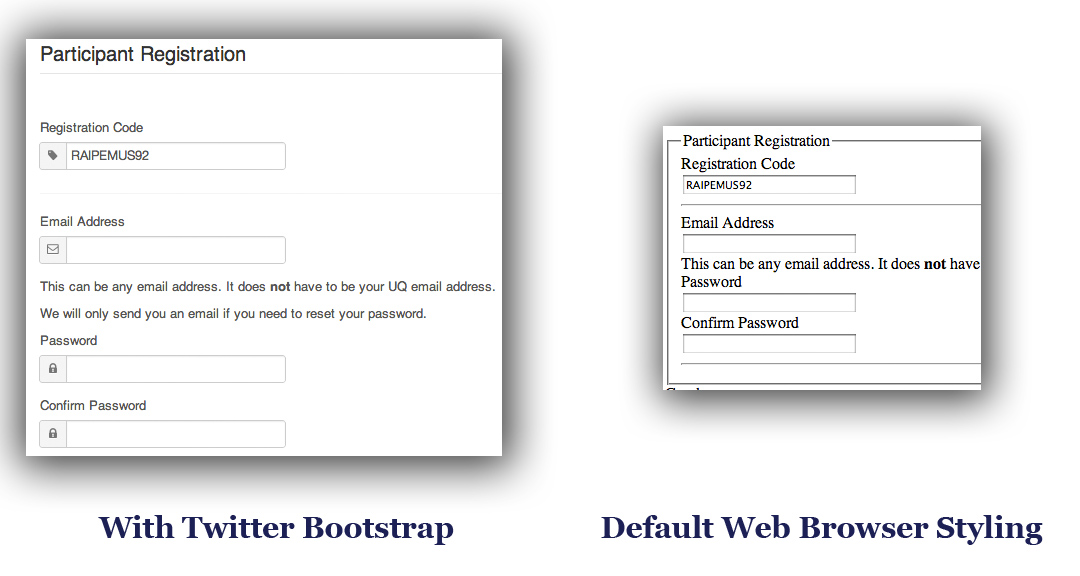
\includegraphics[width=120mm]{img/twitterbootstrap.jpg}
\caption{Comparison of a page with no styling and Twitter Bootstrap default styling}
\label{twitterbootstrap}
\end{figure}

More significantly, Twitter Bootstrap offers a `responsive' layout 
system which provides a reduced screen size (ie. smartphone) layout
 with little to no extra work on the part of the developer. This 
 means a smartphone version of the web application could be designed
  at the same time. Twitter Bootstrap was also chosen for this reason.
  
\paragraph{The R Programming Language}
R is an open source programming language designed primarily for statistical computing. 

\subsubsection{Data Entry}
\subsubsection{Screen Mockups}
\subsubsection{Spaced Repetition Algorithm}
\subsubsection{Data storage, formatting and output}

\subsection{Data Analysis and Prediction}
\subsubsection{R Programming Language}
\subsubsection{Usage Data}
\subsubsection{Forgetting Curves}
\subsubsection{Prediction of Recall}